\documentclass[sigconf]{acmart}
\synctex=1


% Copyright
%\setcopyright{none}
%\setcopyright{acmcopyright}
%\setcopyright{acmlicensed}
\setcopyright{rightsretained}
%\setcopyright{usgov}
%\setcopyright{usgovmixed}
%\setcopyright{cagov}
%\setcopyright{cagovmixed}


% DOI
\acmDOI{10.475/123_4}

% ISBN
\acmISBN{123-4567-24-567/08/06}

%Conference
%\acmConference[WOODSTOCK'97]{ACM Woodstock conference}{July 1997}{El
%  Paso, Texas USA}
%\acmYear{1997}
\copyrightyear{2016}



%=================================================================
% 
\newcount\DraftStatus  % 0 suppresses notes to selves in text
\DraftStatus=1   % TODO: set to 0 for final version
%=================================================================

%=================================================================
\usepackage{comment}
%=================================================================
%
\includecomment{JournalOnly}  
\includecomment{ConferenceOnly}  
\excludecomment{TulipStyle}
%
%=================================================================
%=================================================================
% gitlatexdiff
%
%  https://gitlab.com/git-latexdiff/git-latexdiff
%=================================================================
%  git latexdiff HEAD  HEAD~5 --main templatex.tex
%  git latexdiff HEAD~1  --main templatex.tex
%  View pdf to see difference
%
%=================================================================
%
% Todo Notes for marginal comments
% 
%\newcount\DraftStatus  % 0 suppresses notes to selves in text
%\DraftStatus=1   % TODO: set to 0 for final version
\ifnum\DraftStatus=1
	\usepackage[draft,colorinlistoftodos,color=orange!30]{todonotes}
\else
	\usepackage[disable,colorinlistoftodos,color=blue!30]{todonotes}
\fi 
%\usepackage[disable]{todonotes} % notes not showed
%\usepackage[draft]{todonotes}   % notes showed
%
\makeatletter \providecommand\@dotsep{5} \def\listtodoname{List of Todos} \def\listoftodos{\@starttoc{tdo}\listtodoname} \makeatother
%
%=================================================================
%
\usepackage{color}
\newcommand{\draftnote}[3]{ 
	\todo[author=#2,color=#1!30,size=\footnotesize]{\textsf{#3}}	}
% TODO: add yourself here:
%
\newcommand{\gangli}[1]{\draftnote{blue}{GLi:}{#1}}
\newcommand{\qwu}[1]{\draftnote{red}{QWu:}{#1}}
\newcommand{\gliMarker}
	{\todo[author=GLi,size=\tiny,inline,color=blue!40]
	{Gang Li has worked up to here.}}
\newcommand{\qwuMarker}
	{\todo[author=QWu,size=\tiny,inline,color=red!40]
	{Qiong Wu has worked up to here.}}
%=================================================================

%=================================================================
%
% general packages
%  https://en.wikibooks.org/wiki/Category:Book:LaTeX
%  https://en.wikibooks.org/wiki/LaTeX/Package_Reference
%
%=================================================================
\usepackage{graphicx}
\usepackage{algorithm}
\usepackage{algorithmic}
\usepackage{breqn}
\usepackage{subcaption}
\usepackage{multirow}
\usepackage{psfrag}
\usepackage{url}
\usepackage{hyperref}
%\usepackage[colorlinks]{hyperref}
%\usepackage{cite}
\usepackage{cleveref}
\usepackage{booktabs}
\usepackage{rotating}
\usepackage{colortbl}
\usepackage{paralist}
%\usepackage{geometry}
\usepackage{epstopdf}
\usepackage{nag}
\usepackage{microtype}
\usepackage{siunitx}
\usepackage{nicefrac}
% for random text
\usepackage{lipsum}
\usepackage[english]{babel}
\usepackage[pangram]{blindtext}
% for tikz figures
\usepackage{tikz}
\usetikzlibrary{fit,positioning,arrows.meta,shapes,arrows}
%\tikzset{neuron/.style={circle,thick,fill=black!25,minimum size=17pt,inner sep=0pt},
%	input neuron/.style={neuron, draw,thick, fill=gray!30},
%	hidden neuron/.style={neuron,fill=white,draw},
%	hoz/.style={rotate=-90}}
%
%=================================================================



\begin{TulipStyle}
\usepackage{natbib}
%=================================================================
%
% Version control information
%
%=================================================================
\usepackage{gitinfo2}
%=================================================================
\usepackage{fancyhdr}
\pagestyle{fancy}
\fancyhead{} % clear all header fields
\fancyhead[RO,LE]{\textsl{\rightmark}}
\fancyhead[LO,RE]{\ensuremath{\Rightarrow}
		\textbf{\textbf{[CONFIDENTIAL]}}\ensuremath{\Leftarrow}}
\fancyhead[CO,CE]{}
%=================================================================
\fancyfoot{} % clear all footer fields
\fancyfoot[CE,CO]{\textbf{\thepage}} 
\fancyfoot[LO,LE]{\includegraphics[height=.9\headheight]{logos/tulip-logo.eps}
		\gitVtagn-\gitBranch\ (\gitCommitterDate)}
\fancyfoot[RO,RE]{Committed by: \textsl{\gitCommitterName}}

\setlength{\headheight}{12pt}
\renewcommand{\headrulewidth}{0.4pt}
\renewcommand{\footrulewidth}{0.4pt}
%=================================================================


%=================================================================
% for math notations
% ----------------------------------------------------------------
\usepackage{mathtools}
\usepackage{amsthm}
%
% THEOREMS -------------------------------------------------------
%
\newtheorem{thm}{Theorem}[section]
\newtheorem{cor}[thm]{Corollary}
\newtheorem{lem}[thm]{Lemma}
\newtheorem{prop}[thm]{Proposition}
\theoremstyle{definition}
\newtheorem{defn}[thm]{Definition}
\theoremstyle{remark}
\newtheorem{rem}[thm]{Remark}
\numberwithin{equation}{section}
% MATH -----------------------------------------------------------
\newcommand{\norm}[1]{\left\Vert#1\right\Vert}
\newcommand{\abs}[1]{\left\vert#1\right\vert}
\newcommand{\set}[1]{\left\{#1\right\}}
\newcommand{\Real}{\mathbb R}
\newcommand{\eps}{\varepsilon}
\newcommand{\To}{\longrightarrow}
\newcommand{\BX}{\mathbf{B}(X)}
% ----------------------------------------------------------------
\newcommand{\I}{{\cal I}}
\newcommand{\Id}{{\cal I} }
\newcommand{\Dc}{{\cal D}}
\newcommand{\J}{{\cal J}}
\newcommand{\Dn}{{\cal D}_n}
\newcommand{\Dd}{{\cal D}_n }
\renewcommand{\P}{{\cal P}}
\newcommand{\Nu}{{\cal N} }
\newcommand{\B}{{\cal B}}
\newcommand{\Bf}{{\bf B}}
\newcommand{\Y}{{\bf Y}}
\newcommand{\A}{{\cal A}}
% ----------------------------------------------------------------
\newcommand{\V}{{\cal V}}
\newcommand{\M}{{\cal M}}
\newcommand{\F}{{\cal F}}
\newcommand{\Fd}{{\cal F}}
\newcommand{\BF}{{\cal BF}_n}
\newcommand{\BFd}{{\cal BF}_n}
\newcommand{\TF}{{\cal TF}_n}
\newcommand{\TFd}{{\cal TF}_n}
%\newcommand{\G}{{\cal G}}
\newcommand{\X}{{\cal X}}
\newcommand{\E}{{\cal E}}
\newcommand{\K}{{\cal K}}
\newcommand{\T}{{\cal T}_n}
\renewcommand{\H}{{\cal H}}
% ----------------------------------------------------------------
\newtheorem{Remark}{Remark}
\newtheorem{proposition}{Proposition}
\newtheorem{theorem}{Theorem}
\newtheorem{lemma}{Lemma}
\newtheorem{corollary}{Corollary}
\newtheorem{example}{Example}
\newtheorem{definition}{Definition}
\newtheorem{Algorithms}{Algorithm}
% ----------------------------------------------------------------
\newcommand{\bu}{{\mathbf 1} }
\newcommand{\bo}{{\mathbf 0} }
\newcommand{\N}{\mbox{{\sl l}}\!\mbox{{\sl N}}}
% ----------------------------------------------------------------
\def\uint{[0,1]}
\def\proof{{\scshape Proof}. \ignorespaces}
\def\endproof{{\hfill \vbox{\hrule\hbox{%
   \vrule height1.3ex\hskip1.0ex\vrule}\hrule
  }}\par}
%
%=================================================================

\hypersetup
{
    pdfauthor={\gitAuthorName},
    pdfsubject={TULIP Lab},
    pdftitle={},
    pdfkeywords={TULIP Lab, Data Science},
%	bookmarks=true,  
}

\end{TulipStyle}



%=================================================================
%
\begin{document}
%
%=================================================================
% Preamble which will need to be changed for submission
%
\title{Sentiment Analysis on Movie Reviews}%
% \titlenote{Produces the permission block, and
%   copyright information}
% \subtitle{What is my Subtitle?}
% \subtitlenote{The full version of the author's guide is available as
%   \texttt{acmart.pdf} document}


\author{Yuhui Mou}
% \authornote{Dr.~Trovato insisted his name be first.}
% \orcid{1234-5678-9012}
\affiliation{%
  \institution{Xi'an Shiyou University}
  % \streetaddress{P.O. Box 1212}
  \city{Xi'an}
  \country{China}
  % \postcode{43017-6221}
}
\email{905925264@qq.com}

% \author{Gang Li}
% \authornote{Corresponding Author}
% \affiliation{%
%   \institution{Deakin University}
%   \city{Geelong, VIC 3216}
%   \country{Australia}}
% \email{gang.li@deakin.edu.au}

% The default list of authors is too long for headers.
\renewcommand{\shortauthors}{G. Li et al.}


\begin{abstract}
  Each of us has seen the film,We might write down what we think of it on a movie review website \\
  Film reviews can reflect the quality of films to a certain extent, which depends on the comments of 
  the film critics and their emotions. People who like the film will have good comments,
  while those who don't like the film will have bad comments.Therefore, we can reflect a
   person's feelings based on film reviews.
\end{abstract}
\keywords{Film reviews,BoW,Logistic Regression,\LaTeX, CNN }

\maketitle

%=================================================================
%=================================================================
\section{Introduction}\label{sec-intro}

% Test citation~\cite{BL12J01}. 
% \begin{JournalOnly}
% and~\citep{BJL11J01} or~\citet{BJL11J01}.
% \end{JournalOnly}
The food has its own characteristics of each country.
In this project,we can distinguish different countries by
different ingredients.\\
This is an interesting project.
% \todo[fancyline]{Testing.}
% % and this is for~\cref{sec-conclusions}.
% \todo[noline]{A note with no line back to the text.}%
% \gangli{This is comment from Gang.}
% \qwu{Response from QW}

% Number:
% \num{123}.
% \numlist{10;30;50;70},
% \numrange{10}{30},
% \SIlist{10;30;45}{\metre},
% and
% \SI{10}{\percent}

% \missingfigure[figcolor=white]{Testing figcolor}
% 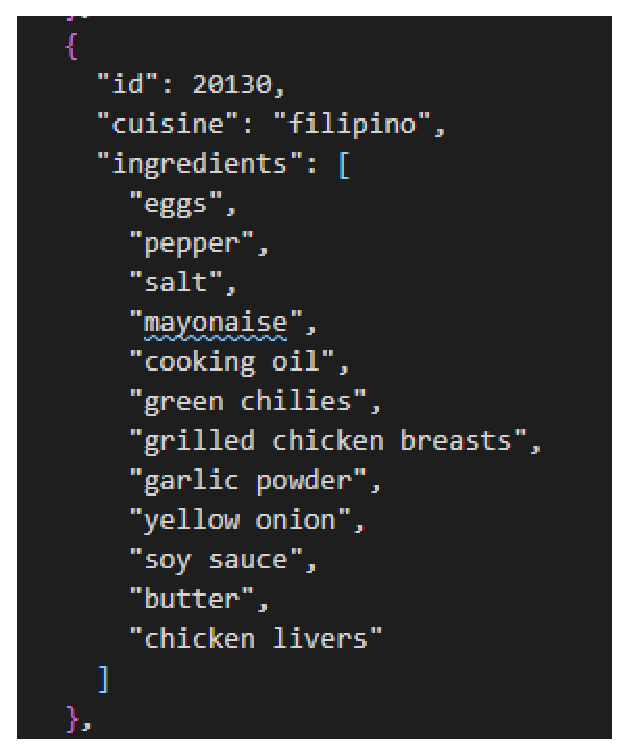
\includegraphics[width=0.4\textwidth]{train.eps}

\includegraphics[width=0.45\textwidth]{D://Code//Kaggle-test//Data//header.png}

% \begin{ConferenceOnly}
% We have \SI{10}{\hertz},
% \si{\kilogram\metre\per\second},
% the range: \SIrange{10}{100}{\hertz}.
% $\nicefrac[]{1}{2}$.

% \missingfigure{Make a sketch of the structure of a trebuchet.}
% \end{ConferenceOnly}
% This is test data\\
% \includegraphics[width=0.4\textwidth]{test-data.png}

% For~\cref{eq:test},
% as shown below:

% \begin{equation}\label{eq:test}
% a = b \times \sqrt{ab}
% \end{equation}
% \begin{minted}{Python}
% 	employees = []
% 	for id in employee_ids:
% 	    employee = fetch_employee(id)
% 	if employee:
% 	    employees.append(employee)
% \end{minted}
% \blindmathpaper

\section{Data} \label{sec-preliminaries}

This event provides two data sets that can be used: train.json  test.json\\
\textbf{train.json}:In the dataset, we include the recipe id, the type of cuisine, and the list of ingredients of each recipe (of variable length). The data is stored in JSON format. \\
\textbf{test.json}:In the test file test.json, the format of a recipe is the same as train.json, only the cuisine type is removed, as it is the target variable you are going to predict.

% \gliMarker  %TODO: GLi Here


\section{Data Processing} \label{sec-method}
\begin{itemize}
  \item
  Read Data \\
  \begin{itemize}
  \item
  Read train.json
  \item
  Read test.json
  \end{itemize}
  \item
  Processing Model:Bag-of-words model (BoW model)\\
  \begin{itemize}
    \item 
    BoW early in Natural Language Processing and Information Retrieval 
    This model ignored the grammar and word order elements such as text, 
    just as it is a collection of several words, the emergence of each
     word in the document are independent of each otherBoW to use an 
     unordered list of words to express a text or a document.
  \end{itemize}
   \begin{itemize}
    \item
    CountVectorizer is a characteristic class of common numerical calculation,
    Is a text feature extraction method.For each training text, it only considers 
    each of these words in the frequency of the training in the text.
    CountVectorizer Converts text of the words in the word frequency matrix.
    It does this by fit_transform function calculating the number of occurrences of all words.
    \end{itemize}
  % \begin{figure}
  %    \selectcolormodel{rgb}
  %    \missingfigure{Make a sketch of the structure of a trebuchet.}
  % %  \includegraphics[width=0.4\textwidth]{figures//example3.eps}\\
  %    \caption{EMD of one feature}\label{EMD}
  % \end{figure}
  \item 
  RandomForestClassifier\\

\begin{itemize}
\item
The first step is using feature and target training classifier.
\item
The second step is to input data to classifier which has trained before.
\item 
Export data and Store them in a document.
\end{itemize}


\end{itemize}
% \blindtext
% \blindlist{itemize}[3]
% \blinditemize
% \blindenumerate

% \blindmathtrue
% \blindmathfalse
% \blinddescription

% \qwuMarker %TODO: QWu Here

% \section{RandomForestClassifier} \label{sec-experiment}


% \begin{table}  \centering
%   \caption{Precision Comparison on Event Detection Methods}
%   \label{tbl:overall-experiments}
%   \begin{tabular}{cccc}
% \toprule
%     % after \\: \hline or \cline{col1-col2} \cline{col3-col4} ...
%     & OR Event Detection & AC Event Detection & TC Event Detection \\
% \midrule
%     precision & 0.83 & 0.69 & 0.46 \\
%     recall & 0.68 & 0.48 & 0.36 \\
%     F-score & 0.747 & 0.57 & 0.4 \\
% \bottomrule
% \end{tabular}
% \end{table}


\section{Conclusions} \label{sec-conclusions}
Every country has its specialties,each cuisine has it's own ingredients.During this competition,I learned how to
identify the country by different ingredients.At the same time, I also learned how to deal with plain text data set-
BoW model,besides,CountVectorizer is also a great way to extracting text feature.In the end,using feature we extarcted to
classify in RandomForestClassifier.



\section*{Acknowledgment}

We want to thank Yummly for providing this unique dataset. Kaggle is hosting this playground competition for fun and practice.

\rightline{
\includegraphics[width=0.15\textwidth]{D://Code//Kaggle-test//Data//Yummly_logo.png}}
The authors would like to thank \ldots


% ----------------------------------------------------------------
% \bibliography{tuliplab,yourbib}
% \bibliographystyle{ACM-Reference-Format}
%=================================================================

\end{document}
